\documentclass[11pt, openright]{book}

    % Cover Variables
    \newcommand{\ctoptitle}{}
    \newcommand{\ctitle}{Title}
    \newcommand{\cautor}{Author}
    \newcommand{\cdate}{day.month.year}
    \newcommand{\sectittle}{Second Title}


    % Header Variables
        \newcommand{\headRE}{Main Topic}
        \newcommand{\headLE}{\emph{\rightmark}}
        \newcommand{\footRE}{Lucas Lescure $-$ \cdate}
        \newcommand{\footLE}{\emph{\thepage}}

    % TOC Variables
        \newcommand{\toctitle}{Table of Content}
        
        \newcommand{\tocchapter}{Chapter}
        \newcommand{\toccount}{3}
  
    % Chapter Variables
        \newcommand{\chvar}{Chapter -}

\usepackage[a4paper, total={16cm, 22.125cm}]{geometry}

% Page Style
\usepackage[]{environ}
% Cover Page 
\usepackage{tikz}
\makeatletter
\def\parsecomma#1,#2\endparsecomma{\def\page@x{#1}\def\page@y{#2}}
\tikzdeclarecoordinatesystem{page}{
    \parsecomma#1\endparsecomma
    \pgfpointanchor{current page}{north east}
    % Save the upper right corner
    \pgf@xc=\pgf@x%
    \pgf@yc=\pgf@y%
    % save the lower left corner
    \pgfpointanchor{current page}{south west}
    \pgf@xb=\pgf@x%
    \pgf@yb=\pgf@y%
    % Transform to the correct placement
    \pgfmathparse{(\pgf@xc-\pgf@xb)/2.*\page@x+(\pgf@xc+\pgf@xb)/2.}
    \expandafter\pgf@x\expandafter=\pgfmathresult pt
    \pgfmathparse{(\pgf@yc-\pgf@yb)/2.*\page@y+(\pgf@yc+\pgf@yb)/2.}
    \expandafter\pgf@y\expandafter=\pgfmathresult pt
}
\makeatother


% Object formatting
\usepackage[12pt]{moresize}
\usepackage[]{anyfontsize}
\usepackage{titlesec}
\usepackage{import}
\usepackage{floatrow}
\usepackage{enumitem}
\usepackage{changepage}
\usepackage[normalem]{ulem}
\usepackage{array}
\newcommand{\ul}[1]{\underline{#1}}

\usepackage[]{chngcntr}
\usepackage{ifthen}
\ifthenelse{\figcountdepth > 1}
  {\counterwithin{figure}{section}\counterwithin{table}{section}}
  {}

\usepackage[format=plain, labelfont=it, textfont=it]{caption}
\makeatletter
\def\@makecaption#1#2{%
    \vskip\abovecaptionskip
    \sbox\@tempboxa{\textit{#1.} #2}

       
   

    \ifdim \wd\@tempboxa >\hsize
        #1. #2\par
    \else
        \global \@minipagefalse
        \hb@xt@\hsize{\hfil\box\@tempboxa\hfil}
    \fi
    \vskip\belowcaptionskip}
\makeatother

\DeclareCaptionFormat{underline}{\uline{#1#2#3}\par}

% Sections
\titleformat{\section}{\fontsize{16}{19.2}\bfseries}{\thesection.}{0.25em}{}
\titleformat{\subsection}{\fontsize{14}{16.8}\bfseries}{\tab\thesubsection.}{0.25em}{}
\titleformat{\subsubsection}{\fontsize{10}{12}}{\uline{\thesubsubsection)\enspace}}{0em}{\uline}





% Geometry

% Typewritting

\setlength{\parskip}{1em}
\setlength{\parindent}{0em}


\newenvironment{items}[3][0pt]
{\def\closesep{#3}
    \vspace{#2}
    \begin{itemize}
        \setlength{\itemsep}{#1}
        \setlength{\topsep}{0pt}
        \setlength{\partopsep}{0pt}}
        {\end{itemize}
    \vspace{\closesep}}

\newenvironment{enum}[3][0pt]
{\defclosesep{#3}
    \vspace{#2}
    \begin{enumerate}
        \setlength{\itemsep}{#1}
        \setlength{\topsep}{0pt}
        \setlength{\partopsep}{0pt}}
        {\end{enumerate}
    \vspace{\closesep}}

\newenvironment{eq}[2]
{\def\closesep{#2}
    \vspace{#1}
    \begin{align*}}
        {\end{align*}
    \vspace{\closesep}}

\newenvironment{lfeq}[2]
{\def\closesep{#2}
    \vspace{#1}
    \begin{flalign*}}
        {\end{flalign*}
    \vspace{\closesep}}
% List Formatting


\NewEnviron{dent}[1]{
    \vspace{-10pt}
    \begin{adjustwidth}{7mm}{}
        \uline{#1}\hspace{2mm}
        \BODY
    \end{adjustwidth}
    \vspace{-10pt}
}


\usepackage[framemethod=tikz]{mdframed}
\newcounter{count_theorem}[section]\setcounter{count_theorem}{0}
\newcommand{\thetheorem}{\arabic{count_theorem}}

\newcounter{count_exercise}[section]\setcounter{count_exercise}{0}
\newcommand{\theexercise}{\arabic{count_exercise}}


\newenvironment{theorem}[1][]{
    \refstepcounter{count_theorem}
    \mdfsetup{
        linecolor=red!30,
        innerbottommargin=10pt,
        linewidth=2pt,
        topline=false,
        bottomline=false,
        rightline=false,
        shadow=true,
        shadowsize=4.5pt,
        frametitlerule=false,
        apptotikzsetting={
                \tikzset{
                    mdfbackground/.append style={
                            left color=red!8,right color=red!3
                        }
                }
            }
    }
    \begin{mdframed}[]\relax
        \ifstrempty{#1}
        {\textbf{Theorem~\thetheorem.} }
        {\textbf{Theorem~\thetheorem.~#1} }
        }
        {\end{mdframed}\vspace{-10pt}
}

\newenvironment{note}{
    \mdfsetup{innertopmargin=5pt,
        linecolor=gray!30,
        linewidth=2pt,
        topline=false,
        bottomline=false,
        rightline=false,
        frametitleaboveskip=0pt,
        shadow=false,
        shadowsize=4pt,
        frametitlerule=false,
        apptotikzsetting={
                \tikzset{
                    mdfbackground/.append style={
                            left color=gray!8,right color=gray!3
                        }
                }
            }
    }
    \begin{mdframed}[]\relax
        \textbf{Note. }
        }
        {\end{mdframed}\vspace{-10pt}
}

\newenvironment{example}{
    \mdfsetup{innertopmargin=5pt,
        linecolor=green!30,
        linewidth=2pt,
        topline=false,
        bottomline=false,
        rightline=false,
        frametitleaboveskip=0pt,
        shadow=false,
        shadowsize=4pt,
        frametitlerule=false,
        apptotikzsetting={
                \tikzset{
                    mdfbackground/.append style={
                            left color=green!7,right color=green!2
                        },
                    mdfframetitlebackground/.append style={
                            left color=green!7,right color=green!2
                        }
                }
            }
    }
    \begin{mdframed}[]\relax
        \textbf{Example. }
        }
        {\end{mdframed}\vspace{-10pt}
}


\usetikzlibrary{calc,arrows}

\tikzset{
    excursus arrow/.style={%
            line width=2pt,
            draw=gray!40,
            rounded corners=2ex,
        },
    excursus head/.style={
            fill=white,
            font=\bfseries\sffamily,
            text=gray!80,
            anchor=base west,
        },
    excursus line/.style={%
            line width=2pt,
            draw=gray!40,
            rounded corners=2ex,
        }
}

\newenvironment{exercise}[1][]{%
    \refstepcounter{count_exercise}
    \mdfsetup{
        singleextra={
                \path let \p1=(P), \p2=(O) in (\x2,\y1) coordinate (Q);
                \path let \p1=(Q), \p2=(O) in (\x1,{(\y1-\y2)/2}) coordinate (M);
                \path [excursus line] ($(O)+(5em,0ex)$) -| (M) |- ($(Q)+(20em,0ex)$);
                \node [excursus head] at ($(Q)+(2.5em,-0.75pt)$) {\ifstrempty{#1}{Exercise \theexercise}{Exercise \theexercise:~#1}};},
        firstextra={
                \path let \p1=(P), \p2=(O) in (\x2,\y1) coordinate (Q);
                \path [excursus arrow,-to] (O) |- ($(Q)+(12em,0ex)$) .. controls +(0:16em) and +(185:6em) .. ++(23em,2ex);},
        middlelinewidth=2.5em,middlelinecolor=white,
        hidealllines=true,topline=true,
        innertopmargin=0.5ex,
        innerbottommargin=2.5ex,
        innerrightmargin=2pt,
        innerleftmargin=2ex,
        skipabove=0.87\baselineskip,
        skipbelow=0.62\baselineskip,
    }
    \begin{mdframed}[]\relax}
        {\end{mdframed}\vspace{-10pt}
}

% Functions and Data Plotting
\usepackage{subfig,wrapfig,adjustbox,multirow}


% Plotting Style
\usepackage{graphicx,pgfplots}
\usetikzlibrary{arrows}
\usetikzlibrary {patterns,patterns.meta}
\usepgfplotslibrary{fillbetween}
\pgfplotsset{compat=1.18}

\usepgfplotslibrary{units}
% Logarithmic Scale
\pgfplotsset{
    log x ticks with fixed point/.style={
            xticklabel={
                    \pgfkeys{/pgf/fpu=true}
                    \pgfmathparse{exp(\tick)}%
                    \pgfmathprintnumber[fixed relative, precision=3]{\pgfmathresult}
                    \pgfkeys{/pgf/fpu=false}
                }
        }
}


% Mathematics

% Formatting
\usepackage{amsmath}
\usepackage{esvect}
\usepackage{amsfonts}
\usepackage{tasks,environ}
\usepackage{xargs}
\usepackage{esint}
\usepackage[]{listings}


\usepackage[english]{babel}
\usepackage{amsthm}
%\newtheorem{theorem}{Theorem}
%\newtheorem{proof}{Proof}



%Custom Shortcuts
\newcommand{\eqi}{\Leftrightarrow}
\newcommand{\lr}[1]{\left( #1 \right)}
\newcommand{\limit}[1]{\displaystyle{\lim_{#1}}}
\newcommand{\tab}{\hspace*{7mm}}
\newcommand{\ds}[1]{\displaystyle{#1}}
\newcommand{\floor}[1]{\lfloor #1 \rfloor}
\newcommand{\R}{\mathbb{R}}
\newcommand{\N}{\mathbb{N}}
\newcommand{\Z}{\mathbb{Z}}
\newcommand{\C}{\mathbb{C}}
\newcommand{\K}{\mathbb{K}}
\newcommand{\F}{\mathcal{F}}
\newcommand{\M}{\mathcal{M}}
\renewcommand{\l}{\lambda}
\newcommand{\seg}[1]{\overline{\rm {#1}}}
\newcommand{\Int}{\int\limits}
\newcommand{\ex}{\tab \uline{Example :}\hspace{0.2cm} }
\newcommand{\vard}{\partial}
\newcommand{\Q}{\mathcal{Q}}
\newcommand{\Vect}{\operatorname{Vect}}
\newcommand{\rg}{\operatorname{rg}}
\renewcommand{\dim}{\operatorname{dim}}
\renewcommand{\Re}{\operatorname{Re}}
\renewcommand{\Im}{\operatorname{Im}}
\renewcommand{\P}{\mathcal{P}}
\newcommand{\blr}[1]{\left\{#1\right\}}
\newcommand{\linecenter}[1]{\par\vspace{2mm} \centerline{#1}\par\vspace{-2mm}}
\newcommand{\dd}{\textrm{d}}
\newcommand{\supp}{\operatorname{Supp}}
\renewcommand{\vec}{\overrightarrow}
\renewcommand{\epsilon}{\varepsilon}

% Matrix Configurations

\makeatletter
\renewcommand*\env@matrix[1][*\c@MaxMatrixCols c]{%
    \hskip -\arraycolsep
    \let\@ifnextchar\new@ifnextchar
    \array{#1}}
\makeatother


% Colors
\usepackage{xcolor}
\newcommand{\blu}{\color{blue}}
\newcommand{\Red}{\color{red}}
\newcommand{\blac}{\color{black}}

\newcommand{\red}[1]{\textcolor{red}{#1}}

\usepackage{xcolor,xspace}
\usepackage{breqn}


% Headings  
\usepackage[Glenn]{fncychap}
\ChNumVar{\fontsize{40}{42}}
\ChTitleVar{\Large\sc}
\ChNameVar{\Large\sc}
\setlength\headheight{14.5pt}
\renewcommand\FmN[1]{\chvar}



\usepackage{fancyhdr}
\usepackage{ragged2e}

% Header & Footers
\renewcommand{\chaptermark}[1]{\markboth{#1}{#1}}
\renewcommand{\sectionmark}[1]{
    \markright{ #1}
}
\pagestyle{fancy}
\fancyhf{}
\fancyhead[LE,RO]{\headLE}
\fancyhead[RE,LO]{\headRE}
\fancyfoot[LE,RO]{\footLE}
\fancyfoot[RE,LO]{\footRE}
\renewcommand{\headrulewidth}{0.5pt}
\fancyheadoffset{1cm}

\fancypagestyle{plain}{%
    \fancyhf{} % clear all header and footer fields
    \fancyfoot[LE, RO]{\footLE}
    \renewcommand{\headrulewidth}{0pt}
    \renewcommand{\footrulewidth}{0pt}}


\fancypagestyle{nohead}{%
    \fancyhf{} % clear all header 
    \fancyfoot[LE, RO]{\footLE}
    \fancyfoot[LO, RE]{\footRE}}

    \fancypagestyle{head}{%
    \fancyhf{} % clear all header 
    \fancyhead[LE,RO]{\headLE}
\fancyhead[RE,LO]{\headRE}
\renewcommand{\headrulewidth}{0.5pt}
\fancyheadoffset{1cm}
    }


\fancypagestyle{bib}{%
    \fancyhf{} % clear all header and footer fields
    \fancyhead[CE, CO]{}
    \fancyfoot[LE, RO]{\footLE}
    \fancyfoot[LO, RE]{Bibliographie}}

% Table of Contents

\renewcommand*\thechapter{\arabic{chapter}} %Usually Roman
\renewcommand*\thesection{\arabic{section}}
\renewcommand*\thesubsubsection{\thesubsection.\alph{subsubsection}}
\makeatletter
\@removefromreset{section}{chapter}
\makeatother


% Table of Contents

\usepackage{titletoc}
\usepackage{ erewhon,cabin}
\usepackage[linktoc=all]{hyperref}
\renewcommand*\contentsname{\centerline{\toctitle}}

\setcounter{secnumdepth}{3}
\setcounter{tocdepth}{\toccount}

\usepackage[subfigure]{tocloft}
\setlength\cftparskip{0pt}

\usepackage{etoolbox}
\makeatletter
\pretocmd{\chapter}{\addtocontents{toc}{\protect\addvspace{5\p@}}}{}{}
\pretocmd{\section}{\addtocontents{toc}{\protect\addvspace{-10\p@}}}{}{}
\pretocmd{\subsection}{\addtocontents{toc}{\protect\addvspace{1\p@}}}{}{}
\makeatother


% Chapter Style
\titlecontents{chapter}
[11em]
{\bigskip}
{\bfseries\textsc\tocchapter~\textsc\thecontentslabel : \textsc}
{\hspace*{-5.5em}\textbf}
{\titlerule*[1pc]{ }}[\smallskip]

% Section Style
\titlecontents{section}
[0em] % i
{\bigskip\bfseries}
{\fontsize{11}{13.2}\bfseries\uline{\thecontentslabel.\enspace}\uline}
{\hspace*{-4em}\textbf}
{\hspace{0.5pt}\uline{\hspace*{\fill}}\contentspage}

% Subsection Style
\titlecontents{subsection}
[2em] % i
{\smallskip\bfseries}
{\fontsize{10}{12}\bfseries\thecontentslabel.\enspace}
{\hspace*{-4em}}
{\titlerule*[0.5pc]{.}\contentspage}

% Subsubsection Style
\titlecontents{subsubsection}
[4em] % i
{\smallskip}
{\fontsize{10}{12}\thecontentslabel)\enspace}
{\hspace*{-4em}}
{\titlerule*[0.5pc]{.}\contentspage}










    % figure support
    \usepackage{import}
    \usepackage{xifthen}
    \pdfminorversion=7
    \usepackage{pdfpages}
    \usepackage{transparent}
    \newcommand{\incfig}[1]{%
            \def\svgwidth{\columnwidth}
            \import{./figures/}{#1.pdf_tex}
    }

    \pdfsuppresswarningpagegroup=1


\begin{document}
% Spacing
% Section Spacing
\titlespacing\section{0pt}{3pt plus 2pt minus 2pt}{6pt plus 2pt minus 1pt}
\titlespacing\subsection{0pt}{0pt plus 1pt minus 1pt}{0pt plus 3pt minus 1pt}
\titlespacing\subsubsection{0pt}{0pt plus 0pt minus 0pt}{0pt plus 2pt minus 0pt}

\usetikzlibrary{shadows}

\newgeometry{left=2.5cm, width=16cm, bottom=2.5cm, top=2.5cm}






% Cover
% Cover
\definecolor{ccolor1}{RGB}{236,145,143}
\definecolor{ccolor2}{RGB}{131,168,192}
\definecolor{ccolor3}{RGB}{182,227,150}
\definecolor{ccolor4}{RGB}{171,206,145}

\usetikzlibrary{fadings}

\begin{titlepage}
    \newgeometry{top=1cm, width=21cm, bottom=1cm}

    \begin{tikzpicture}[remember picture,overlay,every node/.style={anchor=center}]

        \coordinate (Center) at (page cs: 0,-0.5);
        %F4E Logo
        \begin{scope}[scale = 1.5]
            \foreach \angle in {0,30,...,330} {
                    \filldraw[orange!50!yellow,line width=0.01pt,shift=(Center)] (\angle:3.8637) -- (\angle+30:3.8637) -- (0,0) -- (\angle:3.8637);
                    \draw[white, line width = 7pt,shift=(Center)] (\angle:2cm) arc (\angle-60:\angle:2cm);
                    \draw[white, line width = 7pt,shift=(Center)] (\angle+30:2cm) arc (\angle+90:\angle+30:2cm);
                }
            % Outer delimiter
            \foreach \angle in {15,45,...,345} {
                    \filldraw[white, line width = 7pt,shift=(Center)] (\angle:3.8637cm) arc (\angle-15:\angle+45:2cm) arc (\angle+15:\angle-15:2cm) arc (\angle+45:\angle+15:2cm);
                }
            % Inner delimiter
            \foreach \angle in {15,45,...,345} {
                    \filldraw[white, line width = 7pt,shift=(Center)] (\angle:1.0353cm) arc (\angle-75:\angle-45:2cm) arc (\angle+75:\angle+105:2cm) -- (0,0) -- (\angle:1.0353cm);
                }
            % Stars
            \foreach \angle in {0,30,...,330} {
                    \fill[orange!50!yellow,shift=(Center)] (\angle:1.03527cm) -- ++ (231:0.175) -- ++ (33:0.35) -- ++ (177:0.35) -- ++ (321:0.35) -- ++ (105:0.35) -- ++ (249:0.35) -- ++ (33:0.35);
                }
        \end{scope}

        \node[opacity =0.07, inner sep=0pt, anchor=east] at (current page.east){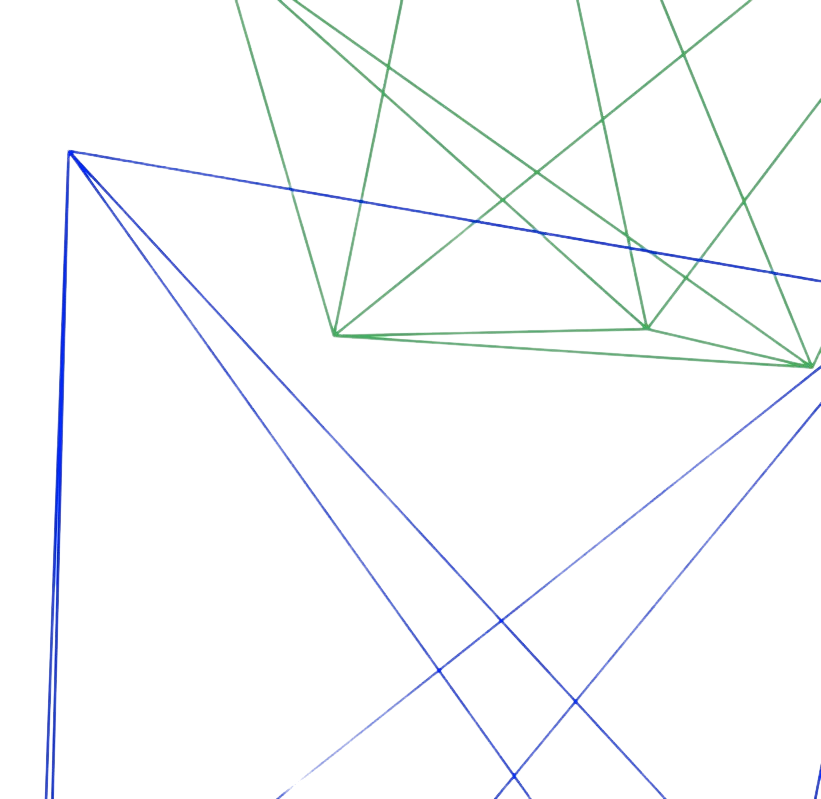
\includegraphics[width=0.5\paperwidth,height=\paperheight]{/root/.config/latex-utils/logos/invert1.png}};

        \node[opacity=0.07,inner sep=0pt, anchor=north west] at (current page.north west){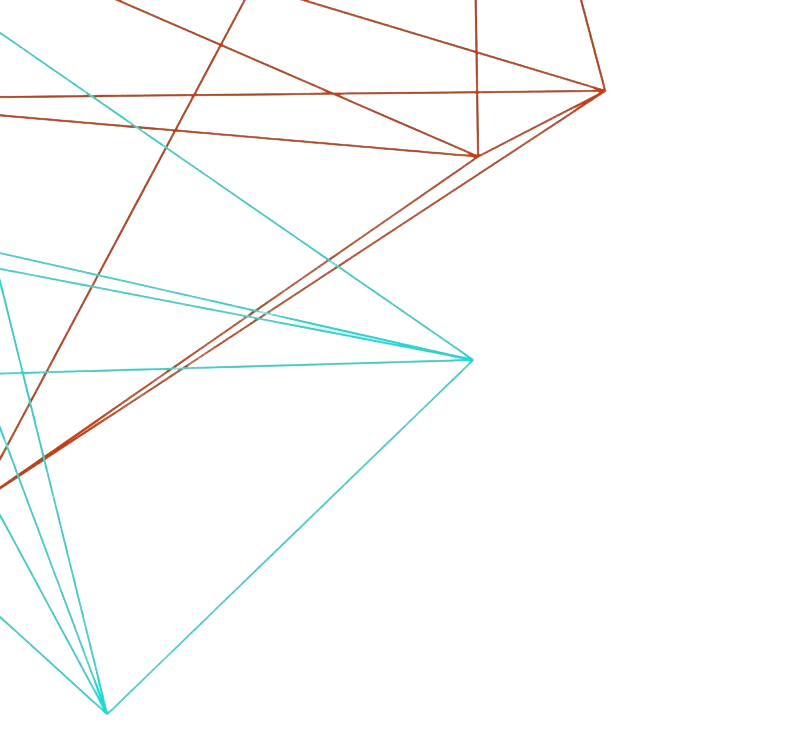
\includegraphics[width=0.5\paperwidth,height=0.5\paperheight]{/root/.config/latex-utils/logos/invert3.png}};




        \node at (page cs:0,0.345) {\Large\textsc{High School Observation and Learning Internship}};
        \node at (page cs:0,0.875) {\Large\bfseries\textsc{Observation Internship}};
        \node at (page cs:0,0.925) {\LARGE\bfseries\textsc{Lycée Français de Barcelone}};

        \node at (page cs:0.5,0) {\Large\textsc{Cyril Lescure - Pedagogical Tutor}};








        %\node[opacity=0.15, inner sep=0pt, anchor=south west] at (current page.south west){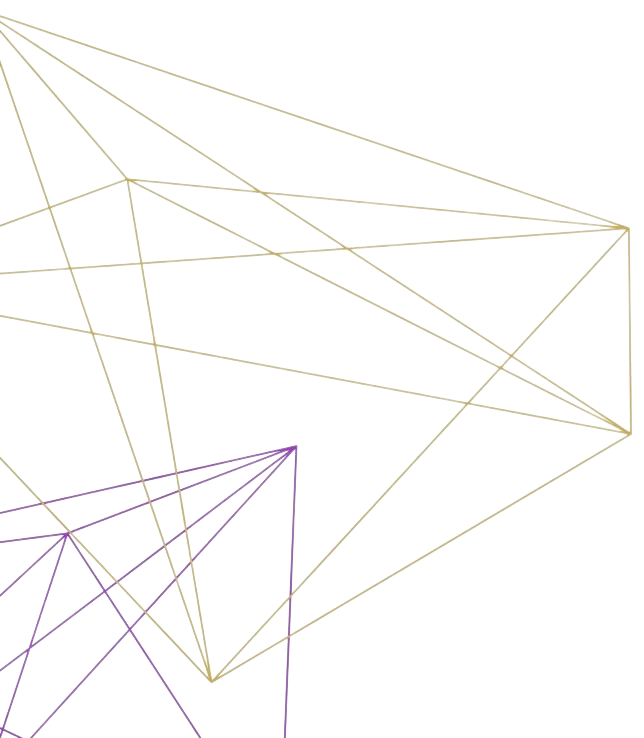
\includegraphics[width=0.5\paperwidth,height=0.5\paperheight]{/root/.config/latex-utils/logos/invert2.png}};

        \node at (page cs:0,0.5) {\fontsize{28}{28.8}\textbf{\ctoptitle}};
        \node at (page cs:0,0.425) {\fontsize{28}{28.8}\textbf{\ctitle}};
        \draw (page cs:0.5,0.375) -- (page cs:-0.5,0.375);
        \node at (page cs:0,0.245) {\LARGE\textsc{\cautor}};
        \node at (page cs:0,0.310) {\Large\textsc{03.06.2019 - 07.06.2019}};


    \end{tikzpicture}
\end{titlepage}


\newgeometry{width=18.625cm, bottom=2cm, top=2cm}

\tikz[remember picture, overlay] \node[opacity=0.3,inner sep=0pt, anchor=north east] at (current page.north east){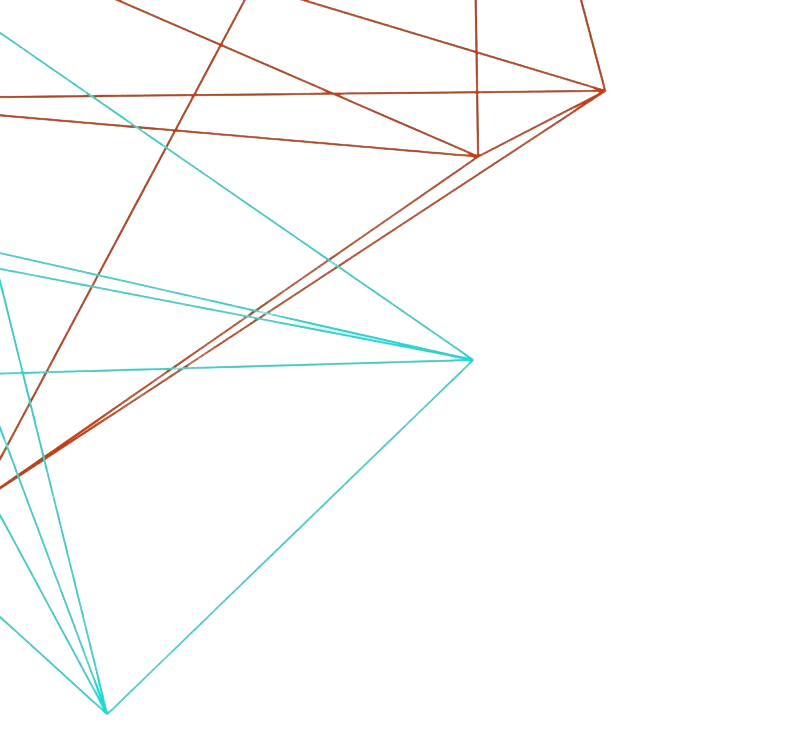
\includegraphics[angle=-90,origin=c,width=0.5\paperheight,height=0.5\paperwidth]{/root/.config/latex-utils/logos/invert3.png}};
\tikz[remember picture,overlay] \node[opacity=0.3,inner sep=0pt, anchor=south east] at (current page.south east){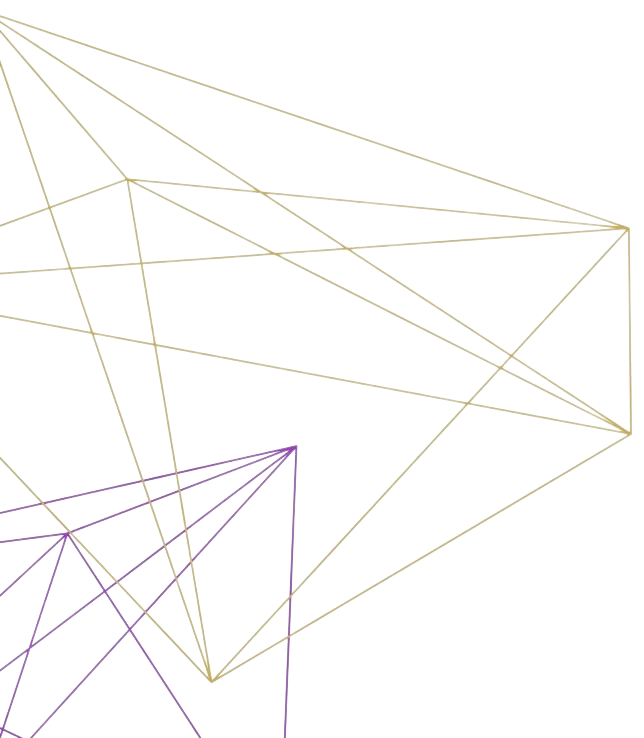
\includegraphics[angle=90,width=0.5\paperwidth,height=0.5\paperheight]{/root/.config/latex-utils/logos/invert2.png}};

\tableofcontents





\newpage

\subsection{convergence in the space of test function D}
A sequence ofo function $\ds{\phi_{k}\in D}$ of functions is said to a function $\ds{\phi \in D}$ when $\ds{k \to \infty}$ if we have :
\begin{dent}{}
    A compact containing the supports of all $\ds{\phi_k}$\\
    $\ds{\phi_k \longrightarrow \phi}$ for $\ds{k \to \infty}$\\
    or $\ds{\phi_k}^{(n)} \longleftrightarrow \phi^{\left(n  \right) }$ for $\ds{k \to \infty}$
\end{dent}

\subsection{Continuous and linear functional T on D}
A linear functional on D is continuous if: for all convergent sequence test function $\ds{\phi_k \to \phi }$ we have:
\linecenter{$\ds{\left< T,\phi_k \right> \to \left< T,\phi \right>  }$}

Definition: "A distribution T is a continuous linear functional on D"
\begin{enum}{-15pt}{-15pt}
    \item If $\ds{\phi}$ is in D then $\ds{\left< T,\phi \right> }$  is a complex number
    \item A distribution is linear operating on test functions  if:
    \linecenter{$\ds{\left< T,\alpha_1\phi_1+\alpha_2\phi_2 \right> =\alpha_1\left< T,\phi_1 \right> +\alpha_2\left< T,\phi_2 \right> }$}
    for test functions $\ds{\phi_1}$  and $\ds{\phi_2}$ and complex numbers $\ds{\alpha_1}$ and $\ds{\alpha_2}$
    \item A distribution is continuous if: $\ds{\phi_n}$ is a sequence of test functions converging to $\ds{\phi}$ then: $\ds{\left< T,\phi_n \right> \to \left< T,\phi \right>  }$
\end{enum}

\subsection{Distribution space D'}
The space of all distributions is denoted by $\ds{D'}$ and is called the dual space of D.

\begin{dent}{Examples and properties:} \\
    Regular distributions:
    \linecenter{$\ds{\left< T_f,\phi \right> =\int\limits_{\R}^{} \phi(x)f(x) \,d x }$}
    $f: \R \longrightarrow \mathcal{C}$, locally intergable function.

    $\ds{\phi}$ has a compact support, so $\ds{f(x)\phi(x)}$ is integrable.

    Question: is $\ds{\left< T,\phi \right> }$ a linear functional?



\end{dent}

\subsection{Distribution: basic idea?}

distributions are a class of linear functions that mapa set of test functions into the set of real numbers. The basic idea in distribution theory is to reinterpret functions as a linear functional acting on a space of test functions by an integral operator:
\linecenter{$\ds{T_f(\phi)=\left< T_f,\phi \right> = \int\limits_{\R}^{} \phi(x)f(x) \,dx  }$}

If $\ds{\phi}$ is a test function, we can use integration by parts to see that :
\linecenter{$\ds{T_f'(\phi)=\left< T_f,\phi \right> =\int\limits_{\R}^{} \phi(x)f'(x) \, dx = -\int\limits_{\R}^{} \phi(x)'f(x) \, d x  }$}

$\ds{f(x)}$ is not differentiable but the corresponding distribtion becomes infinitely differentiable.


\subsubsection{Cauchy principal value}

In mathematics, the Cauchy principal value is a method for assigning values to certain improper integrals which would otherwise be undefined.

When evaluating real integrals of the form $\ds{\int\limits_{a}^{b}f(x)  \,d x }$, $\ds{x}$ real, it is usually assumed that $\ds{f(x)}$ is well defined at all points $\ds{x}$ satisfying $\ds{a<x<b}$.
\linecenter{$\ds{\int\limits_{a}^{b} f(x)  \,d x  = \lim_{\epsilon \to c} \int\limits_{a}^{\epsilon-c} f(x) \,d x +  \int\limits_{\epsilon+c}^{b}  \,d x }$}

Provided the limit exists, the result of the integration may differ for functions undefined at a given point $\ds{c}$, such as $\ds{\frac{1}{x}}$.



\newpage

\section{Chapter 3: Convolution}

\subsection{Introduction}

\subsubsection{PSF}

PSF = Point Spread Function

Any optical system due to optical phenomena will developp a "function d'étalement" caused by aberations, diafragms, etc... Thus in reality when we're observing a point what we obtain is a PSF. When doing these types of measurements what we start to do is measure the impulsional response of the system. The image of an object in the detector is the convolution of the PSF with the true object. The PSF is in the shape of a star as imaged by the detector.


\section{Chapter 4: Convolution Equations}

Let us imagine a Cauchy problem: $f'(t)+\alpha f(t)=0$\\
Where $f(t): \R^+\to \R, f(0)=f_0$\\
Using distribution theory we can consider a casual function $F(t)=H(t)\cdot f(t)$\\
Then we have: $F'(t)=H(t)\cdot f'(t)+\delta f(0)$\hspace{\fill} (for infinitely differentiable functions)\\
We can express $F'(t)=\alpha+F(t)$ as:
\linecenter{$\ds{H(t)\cdot f'(t)+\delta f(0)+\alpha H_(t)f(t)} = \underbrace{H(t)\left( f'(t)+\alpha f(t) \right)}_{=0} + \delta f(0) $}

Conclusion: differential equation express as: \\
\linecenter{$\ds{(\delta' +\alpha\delta)*F=f\circ\delta}$}
Solving differential equations brings the problem to solving a convolution equation.

\subsection{Definition}

Convolution are very useful. Any real instrument will have some impulse response. The measured signal is the result of the convolution of the impulse response with the true signal. Deconvolution is applied to correct this. \\
\linecenter{$\ds{A*\underbrace{X}_{unknown}=B}$}

\subsection{an inverse function}
it is possible to define an inverse for the convolution operator so that a function $A$ convolved by its inverse gives the delta function $\delta$: $A*A^{-1}=\delta$

\subsection{Homogeneous solution}
The homogeneous solution is the solution of the convolution equation when the right hand side is zero:
\linecenter{$\ds{A*X=0}$}

\subsection{The Green function}
constructed as $A*G=\delta$.

Is there a difference between the Green function and the inverse function?

First of all we introduce convolution algebra: A space$\mathcal{A}$ of distribution is said to be "convolution algebra" if it possesses the following properties:
\begin{items}{-15pt}{-15pt}
    \item $\mathcal{A}$ is a vector space
    \item $\mathcal{A}$ is closed under convolution
    \item Convolution is associative for any of the distributions in $\mathcal{A}$
\end{items}

$\mathcal{A}$ is a subspace of $D'$. If $A \in \mathcal{A}$ and $G \in \mathcal{A}$ then $ G=A^{-1}$. $A*X=B$ with $A,B\in \mathcal{A}$.

$X$ is unknown but required to be in $\mathcal{A}$

It is natural to solve the equation by first finding a distribution that is an inverse of $A$: $A^{-1}=\mathcal{A}$ such that $A*A^{-1}=\delta$.\\


Then we can write: $X=A^{-1}*A*X=A^{-1}B$\\
The solution is then: $X=A^{-1}B$\\

\begin{dent}{Theorem:} let us consider $A*X=B$.\\
    The solution is given by $X=X_0+G*B$
\end{dent}

\subsection{Application to an ordinary linear differential equation with constant coefficients}

Mainly to illustrate the technique developed later on. We present a discussion of the problem of solving an ODE:
\linecenter{$\ds{D_n\cdot X(x) = Y(y)}$}
Where $D_n$ is a differential operator of order $n$ with constant coefficients: $\ds{D_n=\sum_{p=0}^{n} a_n \frac{d^n}{dx^n}}$ where $a_n$ are constants.\\

We wish to resolve the equation as a convolution : $d_n*X(x)=Y(y)$.\\

\begin{dent}{Exercise:} $(\delta'-\lambda\delta)^{-1}= ?$ in $\mathcal{D'}^{+}$\\

    $T*(\delta'+\lambda\delta)=\delta$ in $\mathcal{D'}^{+}$ so we knwon thtat $T=H(x)Z(x)$.\\
    $\omega \implies T'-\lambda T=\delta$\\
    $\begin{brace}
            T=H(a)Z(a)\\
            T'=H(a)Z'(a)+\delta Z(0)\\
        \end{brace}$

    $\delta Z(0)+H(a) = \left[ Z'(a)-\lambda Z(a) \right] = \delta $

    $\forall \in \mathcal{D}$

    $\begin{brace}
            Z(0)=1\\
            \underbrace{Z'(a)-\lambda Z(a)}_{Ae^{\lambda a}}=0\\
        \end{brace}$

    $Z(0)=1 \to A=1$

\end{dent}

$d_{n}^{-1}=H(x)\cdot \exp(p_nx)*H(x)\cdot \exp(p_{n-1}x)\ldots$

\begin{dent}{Note: }
    Throught the previous theorem we have used the following property:
    \linecenter{$\ds{(A_1*A_2*A_3*\ldots*A_n)^{-1}}$= ... (missing)}
\end{dent}

\subsection{Integral equation}

Let us consider, for $x>0$ a special form of Valterra's equation:
\linecenter{$\ds{\underbrace{f(x)}_{unknown}+\underbrace{\int\limits_{0}^{x} f(t)\cdot k(x-t) \,d t}_{known} = \underbrace{g(x)}_{known}}$}


Let us write : $F=H\cdot f$ , $G=H\cdot g$, $K=H\cdot k$.\\
The previous equation may be written as a convolution equation $F+K+F=G$ which may be written : $(\delta +K)*F=G$\\
It can be solved by convolving $G$ by the inverse of $\delta +K$.

\subsection{Conclusion}
What are systems?\\

\begin{tikzpicture}
    \draw[] (-1.5,-1) rectangle (1.5,1) ++ (-1.5,-1) node {Systeme};
    \draw[latex-] (-1.5,0) -- (-2.25,0) node[left] {e(t)};
    \draw[-latex] (1.5,0) -- (2.25,0) node[right] {r(t)};
    \node at (0,2) {$r(t)=S(e(t))$};

\end{tikzpicture}

They must respect 3 properties:
\begin{items}{-15pt}{-15pt}
    \item Linearity: $S(\lambda_1e_1+\lambda_2e_2)=\lambda_1S(e_1)+\lambda_2S(e_2)$
    \item Time invariance: if $r(t)=S(e(t))$ then $r(t-t_0)=S(e(t-t_0))$
    \item Continuity: if $e(k)\to e$ then $S(e(k))\to S(e))$
\end{items}

We focus on the class of linear time-invariant systems. With these 3 properties, a rich theory can be developed: Linear Filter.

A linear filter can be uniquely specified by its impulse response $h$ and the output of any filter is mathematically expressed as.



\subsection{Fourier transform of distributions}

Let us consider $\ds{f(x)=H(x)\sin(x)}$. Can we express $I$ the Fourier transform of this function $\ds{f(x)}$ ?
\linecenter{$\ds{I=\int\limits_{-\infty}^{\infty} H(x)\sin(x)e^{-2i\pi ux} \,d x = \int\limits_{0}^{\infty} \sin(x)e^{-2i\pi ux \,d x }}$}

However $I$ does not converge, so the Fourier transform of the function does not exist. What about the Fourier transform of the signal?

$\ds{H(x)\sin(x)}$ is a locally integrable function. So we can link a regular distribution to $\ds{H(x)\sin(x)}$. Otherwise, $\ds{H(x)\sin(x)}$ is a bounded function and the regular distribution linked to a bounded locally integrable function is tempered.
\linecenter{$\ds{\left< T_{H\sin},\phi \right> =\int\limits_{-\infty}^{\infty} H(X)\sin(x)\phi(x) \,d x }$}

\subsection{The n-th dimensional case}
It is possible to extend the Fourier Transform to the function on $\ds{\R_{n}}$ . All properties listed previously can be extended to the n-th dimensional case. The proof is essentially the same as that in the one-dimensional case.
\linecenter{$\ds{\hat{f}(\vec{k})=\int\limits_{-\infty}^{\infty}\int\limits_{-\infty}^{\infty}f(\vec{r})e^{-2i\pi \vec{k}\vec{r}}  \,d \vec{r} }$}

In optics, we can say that a lens applies a Fourier transform. Thus the inverse Fourier transform is also possible by reversing the lens.


\section{Introduction to wavelet transform}

\subsection{Introduction}

While traditional spectral analysis techniques based on Fourier transform or digital filtering provide a good description of stationary and pseudo-stationary signals, they face some limitations when analyzing non-stationary signals.The Fourier transform of $\ds{\cos(2t)+\cos(t)}$ has the same Fourier transform as $\cos(t),\ t<5$ and $\cos(2t),\ t>5$. The Fourier transform does not provide any information on the time at which the frequency changes.

To remedy this problem we can attempt to do it to use a windowed Fourier transform. Which only studies part of the signal. One way to do this is to apply the gate function to the signal upon the studied interval.

\subsection{Windowing: the short time Fourier transform}

The short-time Fourier transform (STFT) is a Fourier-related transform used to determine the sinusoidal frequency of local sections of a signal as it changes overt ime. In practise, the procedure of computing STFT is to divide a longer time signal into shorter segments of equal length and then compute the Fourier transform separately on each shorter segment. This reveals the Fourier spectrum on each shorter segment. One then usually plots the changing spectra as a function of time. %look up par
\linecenter{$\ds{STFT(x(t))= \int_{-\infty}^{\infty} \omega(t-\tau)x(t)e^{2\pi kft}\, dt= \hat{X}(\tau,f)}$}

where $\ds{\omega()}$ is a window function, $\ds{f}$ is the frequency and $\ds{\tau}$ is the time.

\subsubsection{choosing the right width}

One of the pitfalls of the STFT is that it has a fixed resolution. The width of the windowing function relates to how the signal is represented - it determines whether there is good time resolution(the times at which the frequencies change) or not. The narrower the window, the better the time resolution but the worse the frequency resolution. Note the apparition of the Heisenberg uncertainty principle.


The natural question occurs: can there be an optimal windowing function?

We can "contract" in the time domain the function with a "s" factor ( $\ds{s<1}$ ) keeping constant the energy of the signal:
\linecenter{$\ds{f_s(t)=\frac{1}{\sqrt{s}}f(\frac{t}{s})}$}
We can then demonstrate :
\linecenter{$\ds{\int\limits_{-\infty}^{\infty} |f_s(t)|^{2} \,d x = \int\limits_{-\infty}^{\infty}  | f(t)|^{2} \,d x  }$}

In the fourier domain, we have: $\ds{\hat{f_s}(t)=\sqrt{s}\hat{f}(st) }$

More relevant to this chapter, the previous equality determines the trad-off between concentration in one domain and spread in the other; signals concentrated in time will be spread in frequency, and, by duality, signals concentrated in frequency will be spread in time. This is the Heisenberg uncertainty principle.

\subsubsection{Heisenberg uncertainty principle}

Heisenberg Uncertainty principle states that there is inherent uncertainty in the act of measuring a variable of a particle. Commonly applied to the position and the momentum of a particle, the principle states that the more precisely the position is known the more uncertain the momentum and vice-versa : $\ds{\Delta p \cdot \Delta x = h}$ $h$ being the planck constant.



 \subsection{FT transform of a periodic distribution}

 It can be shown that every distibution is tempered and admits a FT of the form: 
 \linecenter{$\ds{\sum_{n=-\infty}^{\infty} C_n\delta(u-\frac{n}{T})}$}

 In other words every periodic distribution of period T has for FT a combination of Dirac whose "teeth" are of unequal length. A periodic function can be written: 
 \linecenter{$\ds{f(x)=F_0(x)*\sum_{n=-\infty}^{\infty} \delta(x-nT)}$}

 What can be written: 
 \linecenter{$\ds{\hat{f}(u)=\hat{f_0}(u)\cdot \sum_{n=-\infty}^{\infty} \frac{1}{T}\delta(u-\frac{n}{T})=\sum_{n=-\infty}^{\infty} \overbrace{\frac{1}{T}\hat{f_0}(u)}^{C_n}\delta(u-\frac{n}{T})}$}

  \subsection{Fourier Series}

  Let a periodic distribution $T(x)$ of period $T$ whose $C_n$ is the Fourier coefficients. This series is the Fourier series of the distribution T:
  \linecenter{$\ds{\hat{T}(u)=\sum_{n=-\infty}^{\infty} C_n\delta(u-\frac{n}{T}) \to T(x)=\sum_{n=-\infty}^{\infty} C_n e^{2i\pi \frac{n}{T}x}$}

  From previously mentioned we remind that $C_n = \frac{1}{T}\hat{f_0}(u)$


  Let us calculate the coefficients $\ds{C_n}$: we have seen that before a periodic function $\ds{f(x)}$ of period $T$ can be written : 
  \linecenter{$\ds{f(x)=f_0(x)=\sum_{n=-\infty}^{\infty} \delta(x-\frac{n}{T})}$}
  
  $\ds{f_0(x)}$ is the elementary pattern ($\ds{f_0(x)=f(x)}$ if $\ds{a<x<a+T}$ and $\ds{0}$ otherwise) : 
  \linecenter{$\ds{\hat{f}(u)=\hat{f_0}(x)\cdot \sum_{n=-\infty}^{\infty} \frac{1}{T}\delta(u-\frac{n}{T})=\sum_{n=-\infty}^{\infty} \frac{1}{T}\hat{f_0}(\frac{n}{T})\delta(u-\frac{n}{T})}$}

  By analogy with the preceding equation: 
  \linecenter{$\ds{C_n=\frac{1}{T}\hat{f_0}(\frac{n}{T})=\frac{1}{T}\int\limits_{-\infty}^{\infty} f_0(x)e^{-2i\pi \frac{n}{T}x} \,d x =\frac{1}{T}\int\limits_{a}^{a+T} f_0(x)e^{-2i\pi \frac{n}{T}x} \,d x }$}

  Note: We believe that we recognise another known result: any periodic function can be developped in Fourier series.

  The above equality has been established in the sens of distributions. This does not, therefore, imply convergence in the sens of the functions of the Fourier series. The latter problem is complex. We admit this result for periodic functions.

  Note: 

  1. We show in the case of a function that the limit of $\ds{C_n}$ when $n$ tands to infinity is equal to $0$. This is false for a distribution.
  
  2. The coefficients which correspond to two opposite values of $n$ are grouped in pairs: 
  \linecenter{$\ds{f(x)=\sum_{n=-\infty}^{\infty} c_n e^{inkx}=C_0+\sum_{n=1}^{\infty} C_n e^{inkx}+ C_{-n}e^{-inkx}= C_0 + \sum_{n=1}^{\infty} a_n\cos(nkx)+b_n\sin(nkx)}$}

  where $\ds{k=\frac{2\pi}{T}}$ 

  With $\ds{\begin{cases}
      a_n=C_n+C_{-n}\\
      b_n=i(C_n-C_{-n})
  \end{cases}}$ therefore : 
  \linecenter{$\ds{a_n}=\frac{2}{T}\int\limits_{a}^{a+T} f_0(x)\cos\left( \frac{2\pi nx}{T} \right)  \,d x $}
  \linecenter{$\ds{b_n}=\frac{2}{T}\int\limits_{a}^{a+T} f_0(x)\sin\left( \frac{2\pi nx}{T} \right)  \,d x $}

   \subsection{Shannon-Whittaker sampling theorem}

   The problem: $\ds{f(x)}$ is a function. We know $\ds{f(a)}$ and $\ds{f(b)}$ and we want to know $\ds{f(x)}$ for $\ds{a<x<b}$. One can choose interpolation formulation, but only an approximate value of $\ds{f(x)}$ is given. %The Shannon-Whittaker sampling theorem gives the exact value of $\ds{f(x)}$.  

   The solution is given by the sampling theorem which offers the possibility of a rigorous interpolation. 

   Theorem: A real function $\ds{f(x)}$ whose TF has a support contained in the interval $\ds{[-U_0;U_0]}$ is completely determined if we know its values at points $\ds{x=nT}$ with : $\ds{n}$ integer and $\ds{T\le \frac{1}{2U_0}}$ 
   
   Proof: To say that one knows $\ds{f(nT)}$ for every integer $\ds{n}$ , amounts to giving ourselves the distribution: 
   \linecenter{$\ds{F(X)=\sum_{n=-\infty}^{\infty} f(nT)\delta(x-nT)}$}
   $\ds{F(x)}$ is the function $\ds{f(x)}$ sampled. 
   \linecenter{$\ds{F(x)=\sum_{n=-\infty}^{\infty} f(x)\delta(x-nT)=f(x)\sum_{n=-\infty}^{\infty} \delta(x-nT)}$} 
   \linecenter{$\ds{\hat{F}(u)=\hat{f}(u)*\sum_{n=-\infty}^{\infty} \frac{1}{T}\delta(u-\frac{n}{T})}$}
   Convoluting the function by a combination of dirac is separating the values one to one by equal lengths.
   
   If $\ds{\frac{1}{T}>2U_0}$ the pattern are separate. \\
   Let us consider : 
   \linecenter{$\ds{\hat{g}(u)=1}$} if $\ds{u\in [-U_0;U_0]}$ and $\ds{\hat{g}(u)=0}$ otherwise. 
   \linecenter{$\ds{\frac{1}{T}\hat{f}(u)=\hat{g}(u)\cdot \hat{F}(u)\implies \frac{1}{T}f(x)=g(x)*\sum_{n}^{} f(nT)\delta(x-nT)}$}
   
   Thus : 
   \linecenter{$\ds{f(x)=T \sum_{n}^{} f(nT)g(x-nT)}$}
   This is an exact interpolation formula.

   Note: we can choose: 
   \linecenter{$\ds{g(x)=\frac{\sin(2\pi U_0x)}{\pi x} \implies \hat{g}(u)=\Pi \frac{u}{2U_0}}$}

   $\ds{\Pi \frac{u}{2U_0}=1}$ for $\ds{|x|<U_0}$ and $\ds{0}$ otherwise.
   
   $\ds{f(x)=\sum_{n}^{} f(\frac{n}{2U_0})\frac{\sin(2\pi U_0x-nT)}{2\pi U_0x-nT}}$
   
   Conclusion: The $\ds{\frac{\sin(x)}{x}}$ function is not the only one that can be used. This procedure shows that one can rigorously determine $\ds{f(x)}$ at any point simply by knowing $\ds{f(nT)}$ for $\ds{n}$ integer.
   
   But the Shannon theorem applies only to certain indefeneitely differentiable functions with unbounded support(since the TF must have a bounded function). In practise these two conditions are not verified. We therefore make an approximation.

    \section{Laplace Transform}

    The Laplace transform is an integral transform named after its discoverer Pierre-Simon Laplace. It takes a function of a real variable $t$ (often time) to a function of a complex variable $s$ (complex frequency). The Laplace transform is very similar to the Fourier transform. While the Fourier transform of a function is a complex function of a real variable (frequency), the Laplace transform of a function is a complex function of a complex variable. Laplace transforms are usually restricted to functions of $t$ with $t > 0$. A consequence of this restriction is that the Laplace transform of a function is a holomorphic function of the variable $s$. Unlike the Fourier transform, the Laplace transform of a distribution is generally a well-behaved function. Also techniques of complex variables can be used directly to study Laplace transforms. As a holomorphic function, the Laplace transform has a power series representation. This power series expresses a function as a linear superposition of moments of the function. This perspective has applications in probability theory.

     \subsection{Laplace transformation of functions}

     Let $\ds{f(t)}$ be a locally summable real or complex function. The bilateral Laplace transform of this function is $\ds{\tilde{f}(p)}$ defined by the complex variable $p$: 
     \linecenter{$\ds{\tilde{f}(p)=\int\limits_{\R}^{} e^{-pt}f(t) \,d t = \mathcal{L_p}[f(t)]}$}.
     
     Note: $\ds{\p\in \mathcal{C}}$ so $\ds{p=a+i\omega}$ where $a$ and $\omega$ are elements of the set of real numbers. So : 
     \linecenter{$\ds{\tilde{f}(p)=\int\limits_{\R}^{} e^{-i\omega t}e^{-at}f(t) \,d t = \mathcal{F_{\frac{\omega}{2\pi}}}[e^{-at}f(t)] }$} 
     
     LT can therefore be understood as teh FT of : $\ds{e^{-at}f(t)}$ 







\end{document}